\subsection{Titles and abstracts} \label{repo_analysis_data}

As mentioned in the introduction, we consider the titles and abstracts of the documents to represent them. In this section, we will present some facts about these two fields, regarding how often they are left empty in the repositories and other noise factors in our corpus, such as the hundreds of texts that are tagged as being written in English when they are not.

\subsubsection{Fill quota}

The title is a required field in all three repositories and is therefore present for all the documents of our corpus. Abstracts, on the other hand, are optional fields. It is empty in 135 of the 7,438 documents of depositonce (1.8 \%), in 922 of the 7,497 documents of edoc (12.3 \%) and in 776 of the 14,464 documents of refubium (5.4 \%). In total, 1,833 of 29,399 documents (6.2 \%) don't have an abstract. Most of the documents that are missing the abstract are publications. None of the 135 documents of depositonce that don't have an abstract are theses. In edoc, only 25 of the 922 documents (2.7 \%) without an abstract are theses; in refubium, 11 of 765 (1.4 \%).

\subsubsection{Foreign languages}

Looking at the data reveals that there are several titles and abstracts which should be written in English (as stated in the tags of the field) but are actually in German. This is the case for 678 titles (2.3 \% of all titles) and 320 abstracts (1.1 \%). Out of the 678 titles, 542 are written in German (80 \%). 381 of these belong to refubium, 90 to depositonce and 71 to edoc. Some titles included in this list are actually in English, but have been misclassified due to their brevity. For example, the two titles that are considered to be written in Polish are ``Przy Bazantarni, Warsaw'' and ``Democrazy ?!''. The second one is clearly not Polish, but given that the word ``Democrazy'' ends like ``Przy'', a misclassification can happen.

Detecting the language of the abstracts is more reliable given the larger size of the text. Out of the 320 abstracts that are not written in English, 319 of them are in German and 1 in Polish. Again, many of the abstracts that are considered to be written neither in German nor English are often in English, but misclassified due to their brevity.

The difference in length between texts written in German and those written in other languages (excluding English) is illustrated in figure \ref{fig:foreign_languages}. German titles comprise 85 characters on average, whereas those in other languages comprise 18 characters. The difference is even more clear when looking at abstracts: German abstracts are 2,682 characters long on average, and those in other languages only 965 characters long. This difference in length supports our hypothesis that texts that are classified as other languages other than German are often errors that occur because of the brevity of the text.

\begin{figure}
    \centering
    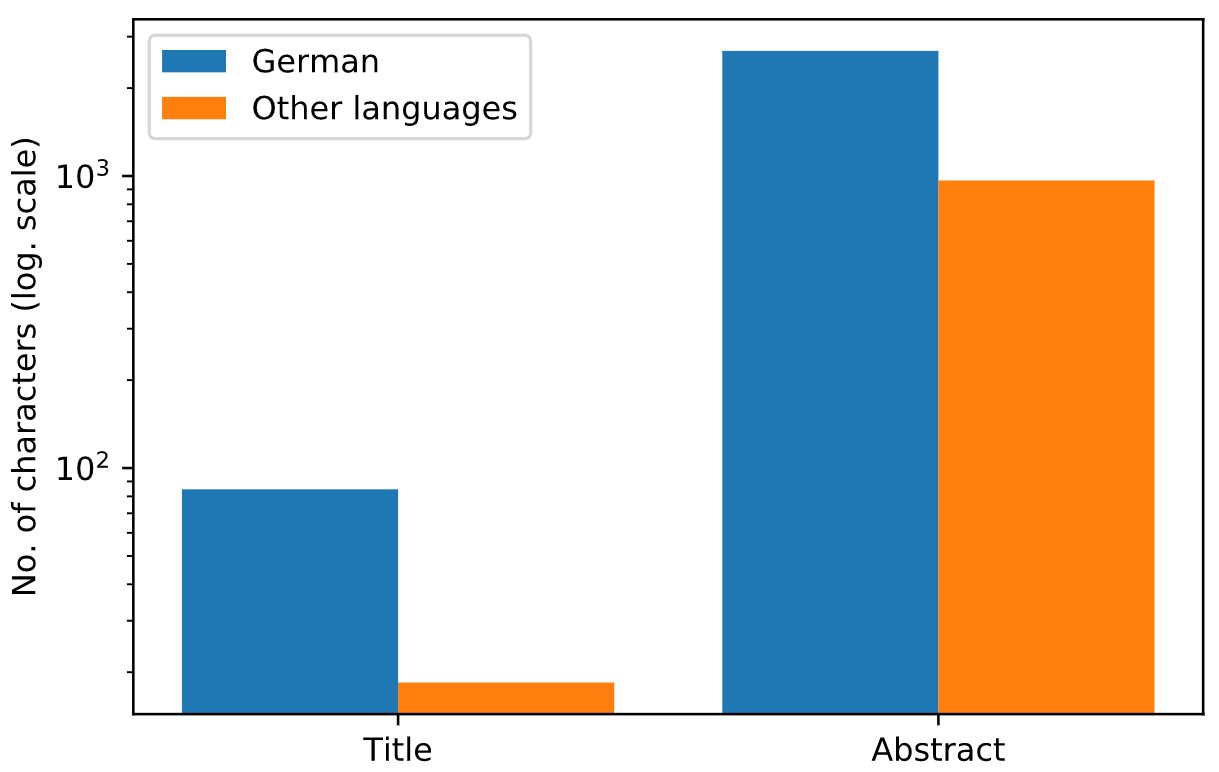
\includegraphics[width=.7\textwidth]{figures/repository_analysis/foreign_languages.PNG}
    \caption{Lengths of titles and abstracts that are not written in English.}
    \label{fig:foreign_languages}
\end{figure}

We determined the language of the texts using the Python package \textit{langdetect}\footnote{\url{https://github.com/Mimino666/langdetect}}, which uses a naive Bayes filter to identify the most probable language out of 53 options. We run the function \textit{detect\_langs} 10 times for each text: a text is written in a foreign language if the probability of the first result is always above 99 \% and the language remains the same throughout all 10 executions. We then use langdetect again to retrieve English texts from the repositories that have been tagged incorrectly (e.g. English texts where the language is said to be German). After extracting all titles and abstracts of each document, we run the language detection procedure described above for each of the possibilities and return the one in English, if any.

Doing so returns English titles for 443 out of the 678 documents (65 \%) with titles in foreign languages and English abstracts for 306 out of the 320 documents (96 \%). When looking at the tags of these retrieved fields, we see that most of them incorrectly state that the text is in German. This is the case for 274 out of the 306 found abstracts. We then run the language detection procedure one again on the improved data. Although we expect to encounter more texts in English, we cannot assume that the number of English texts is now the number of English texts in the original data minus the number of the English texts retrieved with the language detection procedure because of the randomness of the detection model.

This final run shows that 271 titles  (0.9 \%) and 14 abstracts (0.04 \%) are written in foreign languages. 177 of the 271 titles (65 \%) in foreign languages are in German, and all abstracts but one (which is written in Polish) are in German. With this language detection procedure, we have been able to improve the quality of our data, reducing the number of texts written in foreign languages. We have retrieved English texts for 409 titles and 306 abstracts that were previously in foreign languages because of incorrect language tags in the data. 

Please note that these numbers are not fully reliable, given that the model is not always able to correctly predict the language of a text. This can be seen in the number of titles that were deemed to be in foreign languages when looking for alternative titles and those detected in the final run. The first round showed that 235 titles were in foreign languages. Running the same detection procedure again output 271 titles. On the other hand, the detected language for the abstracts remained the same in both runs. This shows that the length of the text is an important factor when evaluating the performance of the language detection model.